\chapter{市场经济体制过渡时期1978--1992年}
\label{chap:1978}

\section{时代背景}

\improve[inline]{在本章或下章加入 向社会主义市场经济过渡}

1976年,毛泽东逝世,党和国家粉碎了四人帮。

据世界银行数据\footnote{\url{https://data.worldbank.org.cn}},1978年的中国GDP总值仅
为1490亿美元,人均GDP(现价美元)156美元,在世界银行所统计的全球130多个国家和
地区中,排名倒数第四,仅高于尼泊尔、几内亚比绍共和国、布隆迪三国,是名副其实
的“\textbf{国穷民弱}”。

本时间段党和国家的改革都基于这一时代大背景。不管是保守派还是自由派的领导人,
都面对一个新时代,只能摸着石头过河,试错是无法避免的。绝大部分人都认为应当否
定阶级斗争为纲,增加民主、尊重价值规律、减轻中央财政负担、引入市场机制、加快
经济建设。但调整幅度多大多小,是保守派和自由派的分歧所在。

\improve{是否是凯恩斯主义?}

\section{整体意识形态转变}

\begin{enumerate}
\item 1978年4月5日,中共中央批转公安部《关于全部摘掉“右派”分子帽子的请示报告
  》,“到1981年,在全面复查的基础上,对错划右派的3改正和落实政策工作全部完成。
  全国共改正错划右派54万人,占原划右派总数
  的98\%”\url{http://www.zgdsw.org.cn/n/2013/0125/c244520-20323571.html}。

\item 1978年5月11日,《光明日报》发表胡福明的文章——《实践是检验真理的唯一标
  准》,新华社转发。次日《人民日报》和《解放军报》同时转载,拉开了全国范围内
  极左路线失势的序幕,华国锋“两个凡是”理论倒台。

  % 笔者认为需要说明的是,不考虑本文背后的社会和政治意义,其中的理论本身大部分是正
  % 确的,也是马克思一直坚持的,他所关注的是实践中的人和社会,正是这种实践的要求,
  % 要求理论与时俱进,要求马克思主义理论对其自身的批判和发展。也正因此,马克思抛弃
  % 了形而上学的终极实存的哲学体系,也同时抛弃了纯粹的、试图超越人类历史和实践的自
  % 然辩证法,他所提倡的是成为运动的、实践的、历史的、辩证的、人的历史唯物主义,并
  % 试图改造世界以此让世界更加美好。但胡福明此文错在“唯一标准”,这是一种过度扩展,
  % 有损于马克思的严谨审慎。笔者再次重申,马克思科社思想仍未脱离空想社会主义范畴,
  % 这使其成为乌托邦。
  % 详情请见\cref{sec:marxkexue}一节。

\item 1978年11月10日--12月15日,在北京召开中央工作会议,原定议题讨论经济。陈云在
  东北组率先提出系统解决历史遗留问题,平凡一系列重大冤假错案(“到1982年底,
  约有300多万名干部得到平反。”);邓小平提出“再不实行改革,我们的现代化事业
  和社会主义事业就会被葬送”。1978年12月13日,邓小平总结发言《解放思想,实事
  求是,团结一致向前看》,提到反官僚主义、加强责任制、“允许一部分地区、一部
  分企业、一部分工人农民,由于辛勤努力成绩大而收入先多一些,生活先好起来”,
  同时对落后地区和人民给以有力支持等等。

\item 1978年12月18日至22日,中共十一届三中全会在北京召开,继承了几天前的中央工作
  会议精神,另外“邓小平实际上已成为中央领导集体的核心。”。本次会议是纠正极
  左路线、发展市场经济的一个重要转折点,全党工作重点转移到社会主义现代化建设
  上来。

\item 1981年6月27日至29日,中共十一届六中全会在北京召开,会议一致通过《关于建国
  以来党的若干历史问题的决议》,由党和政府系统梳理了这段历史,论述功过,极左
  势力下台。

\item 1981年9月30日,叶剑英继承和发展了毛泽东、周恩来所提出的“一纲四目”,进一
  步阐明关于台湾回归祖国,实现和平统一的9条方针政
  策, 提出“(3)国家实现统一后,台湾可作为特别行政区,享有高度的自治权,并可保留军
  队。中央政府不干预台湾地方事务。(4)台湾现行社会、经济制度不变,生活方式不变,
  同外国的经济、文化关系不变。”1982年,邓小平就叶剑英谈话指出,这实际上就
  是“一个国家,两种制度”。“一国两制”随后也成为香港、澳门回归中国的重要指
  导思想。邓小平在港澳回归问题上立场坚定,行动果决。

\item 1982年1月25日,农历正月初一,陈云约请国家计委负责人座谈,强调计划经济为主、
  市场经济为辅。“计划派”暂居“改革派”上风。

\item 1982年9月1日,邓小平在中共第十二次全国人民代表大会开幕式上致开幕词,首次提
  出“\textbf{有中国特色的社会主义}”,开创了全面转向社会主义现代化建设的新局面。
  \begin{quotation}
    我们的现代化建设,必须从中国的实际出发。无论是革命还是建设,都要注意学习和借
    鉴外国经验。但是,照抄照搬别国经验、别国模式,从来不能得到成功。这方面我们有
    过不少教训。把马克思主义的普遍真理同我国的具体实际结合起来,走自己的道路,建
    设有中国特色的社会主义,这就是我们总结长期历史经验得出的基本结论。

    八十年代是我们党和国家历史发展上的重要年代。加紧社会主义现代化建设,争取
    实现包括台湾在内的祖国统一,反对霸权主义、维护世界和平,是我国人民在八十
    年代的三大任务。这三大任务中,核心是经济建设,它是解决国际国内问题的基
    础。
    \footnote{\url{http://cpc.people.com.cn/GB/64162/64168/64565/65448/4429495.html}}
  \end{quotation}

\item 1982年,黄克诚向陈云提出“要把经济搞活,不能再像过去那样搞死,但搞活不能没有
  秩序。这就好比一只鸟,不能捏在手里,捏在手里它就死了,要让它飞。但要让它在笼子
  里飞,否则它就飞跑了。”陈云在之后两三个月里反复引用了黄克诚的谈话,并且加以
  补充:“搞活经济是对的,但必须在计划的指导下搞活。” 后被称为“\textbf{鸟笼经济}”,
  此鸟笼与我们当前的“\textbf{腾笼换鸟}”完全不同。陈云此时的“笼子”强调的是计划经济
  的约束,我们今天的笼子强调的是空间生产。\cite{niaolongjingji}

\item 1983年10月党的第十二届中央委员会第二次全体会议通过了关于整党的决定,邓小平
  在会上讲话,强调整党不能走过场,要清理“三种人”(指在“文革”中追随林彪、
  江青反革命集团造反起家的人;帮派思想严重的人;打砸抢分子)。1984年6月30日,
  中共中央整党工作指导委员会发出第9号通知,明确强调要进行彻底否定“文革”的教
  育。\footnote{\url{http://l.zhuixue.net/jindai/89487.html}}

\item 1984年10月20日,中共第十二届三中全会通过重要纲领性文件《中共中央关于经济体
  制改革的决定》。《决定》中指出“改革计划体制,首先要突破把计划经济同商品经
  济对立起来的传统观念,明确认识社会主义计划经济必须自觉依据和运用价值规律,
  是\textbf{在公有制基础上的有计划的商品经济}。……就总体说,我国实行的是计划经济,
  即有计划的商品经济……改革过分集中的价格管理体制,逐步缩小国家统一定价的范
  围,适当扩大有一定幅度的浮动价格和自由价格的范围。”此外《决定》还涉及城市
  重点转移、价格改革、政企职责界定等。本文对于这些内容的探讨将分别放在下述相
  关章节。

  张曙光评价
  \begin{quotation}
    \textbf{这样,“有计划的商品经济”代替了“计划经济为主,市场经济为辅”。成为中
      国经济体制改革的目标模式。}
  \end{quotation}

\item 1986年9月28日,中共十二届六中全会通过《中共中央关于社会主义精神文明建设
  指导方针的决议》。《决议》中指出:
  \begin{quotation}
    我国社会主义现代化建设的总体布局是:以经济建设为中心,坚定不移地进行经济体制
    改革,坚定不移地进行政治体制改革,坚定不移地加强精神文明建设,并且使这几个方
    面互相配合,互相促进。\footnote{\url{http://cpc.people.com.cn/GB/64162/64168/64565/65381/4429515.html}}
  \end{quotation}

\item 1987年10月25日,赵紫阳在中共第十三次代表大会报告《沿着有中国特色的社会主义
  道路前进》中提出
  \begin{quotation}
    \textbf{社会主义初级阶段}不是泛指任何国家进入社会主义都会经历的起始阶段,而是特
    指我国生产力落后、商品经济不发达条件下建设社会主义必然要经历的特定阶段。
    即从1956年社会主义改造基本完成到21世纪中叶社会主义现代化基本实现的整个历
    史阶段。

    我国正处在社会主义的初级阶段。这个论断,包括两层含义。第一,我国社会已经是社
    会主义社会。我们必须坚持而不能离开社会主义。第二,我国的社会主义社会还处在初
    级阶段。我们必须从这个实际出发,而不能超越这个阶段。在近代中国的具体历史条件
    下,不承认中国人民可以不经过资本主义充分发展阶段而走上社会主义道路,
    是\textbf{革命发展问题上的机械论},是右倾错误的重要认识根源;\textbf{以为不经
      过生产力的巨大发展就可以越过社会主义初级阶段,是革命发展问题上的空想
      论},是“左”倾错误的重要认识根源。
  \end{quotation}

  严立贤就此报告中的“\textbf{政府调控市场,市场引导企业}”写到
  \begin{quotation}
    在十二届三中全会,只是强调国家计划必须依据价值规律,而在这里,\textbf{国家计
      划必须通过市场来实现},也即只能通过市场把企业引导到国家计划上来。这
    样,\textbf{指令性计划必然要退居次要位置},整个经济体制因此向市场经济迈进了一
    大步。 \footnote{\url{http://jds.cass.cn/ztyj/jjs/201605/t20160506_3324987.shtml}} \end{quotation}

  在马克思所作的科学共产主义重要纲领性文献《哥达纲领批判》中,将共产主义分为
  共产主义初级阶段(即社会主义)和共产主义高级阶段,初级阶段是向高级阶段的过
  渡期。“社会主义初级阶段”其实并不如报告中所说“已经进入社会主义社会”。它
  不是“共产主义初级阶段”——社会主义,而是相较社会主义阶段带有更多资本产权、
  法权性质的“前社会主义阶段”。


  事实上,不管苏俄或者中国如何左或如何宣称,都始终都未曾脱离国家资本主义主体
  的范畴,列宁在战时共产主义失败后对此具有较为清醒认识。在社会主义国家阵营的
  实践中,马恩历史唯物主义中所说的“物质生活条件、生产关系和交换关系的发展程
  度”确实是无法跨越的卡夫丁峡谷。这次大会可说是理论准确。

  赵紫阳本次大会报告上提出\textbf{“一个中心”——以经济建设为中心,将坚持四项基本原
  则和坚持改革开放列为两个基本点。} 据赵紫阳《改革历程》记载,邓力群、胡乔木、
  王忍之等保守派在中共十三大之前对“一个中心,两个基本点”意见较大,他们认为
  应当坚持“四项基本原则为纲,改革开放为目”。自由派居保守派上风。

  据张曙光,“我国处于什么样的阶段”的最早争论始自1979年2月5日苏绍智、冯兰瑞
  在理论工作务虚会上的报告《无产阶级取得政权后的社会发展阶段问题
  》。\pagescite[][258-266]{fengyunshi1a}

\item 1988年9月26日至30日,中共十三届三中全会召开,“会议批准了中央政治局向这次全
  会提出的\textbf{治理经济环境、整顿经济秩序、全面深化改革}的指导方针和政策、措
  施。……治理经济环境,主要是压缩社会总需求,抑制通货膨胀。整顿经济秩序,就是要
  整顿目前经济生活中特别是流通领域中出现的各种混乱现
  象。
  ”\footnote{\url{http://cpc.people.com.cn/GB/64162/64165/70293/70319/4857100.html}}

  试图使市场计划与市场双轨快速并轨的价格改革彻底失败,保守派势力相较之前有所增强,
  自由派势力受到暂时抑制。

\item 1992年1、2月,邓小平南巡讲话。1992年6月9日江泽民在中央党校省部级干部进修班
  上作《深刻领会和全面落实邓小平同志的重要谈话精神,把经济建设和改革开放搞得
  更快更好》的讲话,提出当前在建立新经济体制问题的认识上目前有三种提
  法——“\textbf{计划与市场结合的社会主义商品经济体制}”、“\textbf{社会主义有计划的市场
    经济体制}”和“\textbf{社会主义的市场经济体制}”。“我个人的看法,比较倾向于使
  用‘\textbf{社会主义市场经济体制}’这个提法”。1992年10月的中共十四大上,江泽民明
  确提出:中国经济体制的改革目标是建立\textbf{社会主义市场经济体制}。中国改革开放的
  步伐由此进一步加快。中国正式进入市场经济时期。
\end{enumerate}

\section{领导制度改革}


1980年8月18日,邓小平在中共中央政治局扩大会议上作了《党和国家领导制度的改革》
的讲话。“陈云同志提出,我们选干部,要注意德才兼备。所谓德,最主要的,就是坚
持社会主义道路和党的领导。在这个前提下,干部队伍要\textbf{年轻化、知识化、专业化},
并且要把对于这种干部的提拔使用制度化。这些意见讲得好。”,要求\textbf{废除干部领导
  职务终身制,建立退休制度}和发扬“社会主义民主制度和党的民主集中
制”。\url{http://news.12371.cn/2017/03/09/ARTI1489054449475294.shtml}
\begin{quotation}
  本次会议对中国政治体制中的“官僚主义”、“权力过分集中”的弊端进行了严厉批
  判,将部分过往的政治内容划为封建专制主义,首次提出“改革党和国家领导制度及
  其他制度”的问题。这篇讲话,后来被中共十三大认为是“中国政治体制改革的纲领
  性文献”,也被党内外的主流研究者们奉为研究邓小平政治体制改革思想的经
  典。\footnote{\url{http://www.yhcqw.com/33/9626.html}}
\end{quotation}

1982年1月13日,邓小平在中共中央政治局会议上作了《精简机构是一场革命》的重要讲
话,贯彻和加强了领导制度改革。此后各级机关进行了大规模精简、建立干部离退休制
度等。1985年到1987年,中国人民解放军也裁军百万。

1982年12月4日全国人大五届五次会议通过并施行的《中华人民共和国宪法》规定全国人
大委员长、副委员长,中国人民共和国主席、副主席,国务院总理、副总理、国务委员,
最高人民法院院长,最高人民检察院院长连续连任不得超过两届。彭真在本次大会所作
宪法修改草案报告中就此项规定说,“这就取消了实际上存在的\textbf{领导职务的终身制}。”


1982年9月召开的中共十二大会议上通过了1982年版的《中国共产党章
程》\footnote{\url{http://guoqing.china.com.cn/2012-09/05/content_26433894.htm}},决
定设立中央和地方各级顾问委员会。有相当资历和成绩的老党员、老人进入顾问委员会;
中顾委接受中央委员会的领导,但具有建议、协调、监督、宣传等权利。

笔者认为设立中顾委的本意明确,确实如邓小平在9月13日举行的中顾委第一次会议上所
说
\begin{quotation}
  中央顾问委员会是个新东西,是根据中国共产党的实际情况建立的,是解决党的中央
  领导机构新老交替的一种组织形式。目的是使中央委员会年轻化,同时让一些老同志
  在退出第一线之后继续发挥一定的作用。……是一种过渡性质的组织形
  式。\footnote{\url{http://www.qstheory.cn/books/2016-08/31/c_1119485398_2.htm}}
\end{quotation}

中顾委委员和地方顾问委员会委员人选富有流动性,老顾问委员定期批量退休,部分较
老的一线官员再退出一线工作增补进来,并且这种流动性与日俱增。1986年10月,彭真、
邓颖超、徐向前、聂荣臻四老“\textbf{全退}”,不再担任任何职务。邓小平、陈云、李先念
三老“\textbf{半退}”,仍担任一定职务。1989年9月,邓小平明确提出十四大以后不再设立
顾问委员会。1992年10月18日,中共第十四次全国代表大会通过了关于中央顾问委员会
工作报告的决议,大会同意不再设立中央顾问委员会。中顾委完成了它的历史使命。

就政治利益而言,在邓小平1978年事实上成为核心领导人之际,仍有一些与他相近资历
却未必意见一致的老人。邓小平通过扶持对经济开放持激进态度的年轻领导班子,制衡
拥有巨大权力的幕后老人——尤其是希望放缓改革开放步伐的保守派老人。通过中顾委
改革的进行,政坛老人的影响力和权力逐步减弱,邓小平成为实际上的“一个婆婆”,
为其执政思想方针的实施打下坚实基础。

老人政治具有相当弊端,个人威权较大,给予民主的空间少,容易因循守旧、权欲过强,
人治为上。拥有极大魄力的邓小平试图去革除这一弊端,但是在现实的实施上,最后仍
然走向“一个婆婆”,由统治者个人决定了时代走向。

就“民主集中制”方面,一个良好的中国“民主集中制”因中国历史和现实问题必然不
是西方口头宣传唬烂的那一套民主。如何在保障集中制为主的基础上加强民主和法治成
分,邓小平前行了几大步,大力推动党和领导制度改革,废除领导干部终身制,功绩不
能抹杀。虽未探索出最终的道路,但不能对他过于苛责。

\section{党内分歧}

% 本节内容主要参考了赵紫阳回忆录《改革历程》。本书由杜导正作序,鲍彤导言,萧洪
% 达、姚锡华、杜星垣、杜导正根据赵紫阳下台后的录音整理而来,涉及十一届三中全会
% 以来至90年代的历史变革及政坛风云。因此回忆录并非赵紫阳亲笔独立完成,一些意见
% 看法可能代表整理者看法,还请读者慎重对待。

% 笔者个人认为,赵紫阳在本书中所表现出来的宏观理论、思想认识水平令人意外地浅薄,
% 一些设想远远漂浮于上天,且将一些政坛风云变幻写成了百姓家常。这可能有以下几个
% 原因:1,不便深入;2,赵紫阳年老衰退;3,一些资料因权限问题无法查证,赵紫阳在
% 书中也有提及这点;4,因出版和社会形势压力有所删节,避重就轻;5,赵紫阳本人确
% 实水平有限;6,整理者问题;7,其它。笔者更倾向于第5条是主因,也就是最高职位曾
% 达至中共中央总书记的赵紫阳政治、水平与位置严重不相匹配。考虑时局,邓小平之所以重
% 用“年轻”的胡耀邦、赵紫阳,或许也因他们各方面思想认识水平上同样“年轻莽
% 撞”吧。

\improve[inline]{基建起因、发展、结果。据《改革历程》一书,陈云支持大幅削减基建,
  赵紫阳支持软着陆。}

这一阶段最主要的党内分歧是:以邓小平代表的自由派倡导更全面些的改革开放,以经
济建设为中心;以陈云为代表的保守派倡导计划经济调控下的有限开放;两任中共中央
总书记胡耀邦、赵紫阳都属于自由派,作为有闯劲的“年轻领导人”压制保守派。

关于自由派与保守派的斗争具体路径如下:

1980年5、6月讨论制定六五计划时,陈云提出确保财政平衡、信贷平衡,为此可放缓经
济增速,大大压缩基建规模、预防财政赤字、通货膨胀。

邓小平支持大力开放经济特区、吸引外资;陈云对沿海地区资本和外资投机较为警惕,
对资本的唯一目的是超额利润保持警惕,对特区有意见,希望任用的沿海领导人更为思
想坚定而不是“头脑灵活”。赵紫阳回忆录中认为1981、1982年对沿海地区经济领域犯
罪的打击由陈云主导,有扩大化的错误,有碍于改革开放进程。

1984年因经济发展速度过快、信贷发放过猛、过多,基建规模过大,导致通货膨胀。陈
云支持大缩基建和财政赤字,赵紫阳支持较为柔和的软着陆。

% 多种资料中认为胡耀邦作为党和国家高层领导人,缺乏与职位相相称的老成持重和政治、
% 经济知识,好大喜功。另一方面,胡耀邦个人身上似乎有着唐吉坷德式的理想色彩,并
% 敢于为理想以身犯险,他的支持者和反对者往往都一致高度赞誉他的个人品德,笔者也
% 不例外。问题是胡耀邦作为党和国家领导大德小能,这在各国政坛来说都很难有好结局,
% 这种失衡也不比其他错配更加优越,同样可能对国家和人民造成极大和无可挽回的恶
% 果。

胡耀邦对产值和经济发展速度不是一般乐观,漠视财政赤字和通货膨胀,和陈云意见两
极。

因社会变革,民间人心的激荡与彷偟;因对往过的反思,知识界首先开始探讨毛时代人
道主义的缺失;因权力寻租、官僚腐败、经济通膨等问题民间也有反对声音。至始至终,
胡耀邦对知识界自由一向抱有支持态度,在1983年批判了邓力群等激进左派所要求
的“清除精神污染”运动,与激进左派矛盾加深。后来在反对“资产阶级自由化”问题
上,与党内实权老人产生激烈矛盾,成为其下台的根本原因。据林牧《习仲勋晚年的几
件大事》回忆,这一时期支持胡耀邦的高层领导人有赵紫阳、习仲勋、李先念和万里。

赵紫阳认为邓小平与胡耀邦决裂的根本原因是胡耀邦相对支持资产阶级自由化。当时民
间有些声音要求“民主”政治,以一些高校师生为代表。1985年9月18日,北京85学潮时
有个别学生打出了反对邓小平、胡耀邦的口号。胡耀邦对此不太在意,邓小平意见较
大。

1986年9月十二届六中全会闭幕时,陆定一不支持资产阶级自由化的提法,认为这是文革
时整人的提法,王震、薄一波主张反对资产阶级自由化,对此胡耀邦的表态模棱两可,
邓小平作最后发言时批评了陆定一。赵紫阳认为胡耀邦此时的表现已经意义不大,因为
在此之前邓已经决定拿下胡。

86年末全国一些城市兴起学潮。1987年1月1日,北京学生游行。1月2日,当局释放被关
押人士,游行结束,这成为压倒胡耀邦的最后一根稻草。

反对资产阶级自由化其实就是坚持我党一党专政。反对“资产阶级自由化”不能简单等
同于反对民主,不能说是全错或只为维持权贵利益。我国古今历史主流中从未出现过这
样一种民主体制。笔者始终认为,中国目前仍要坚持民主的集中制,民主为辅,集中制
为主。\footnote{笔者对为何要坚持民主集中制的探讨将放在“关于中国”这一部份的结论部分
  详细探讨,不在此赘述。}但是民主成分如何参与到集中制来,特别是民众的民主而非
高层领导人之间的民主,这是中国仍需具体问题具体分析的特重大问题,并且对这一问
题的理智探讨会艰辛和困难。民主是好的,但空喊口号太容易,具体落实怎么办?中间
会出现什么样的问题?直至今日,个别“进步”学生和师生仍存在着心中激情满满、脑
中空空荡荡的严重缺陷,不考虑历史现实。

胡耀邦下台的另一个根本原因就是老人“退不退”的问题。1985年胡耀邦与时任香港
《百姓》杂志主编陆铿谈话时以及86年访欧及与四川省代表谈话时,在老人们“退不
退”问题的回答上表现不力。

在1987年1月追究胡耀邦错误,致使胡耀邦辞职的会议上,有人率先就老人“退不退”的
问题发难胡耀邦,这在中国历朝历代都是诛心之论。这个人是谁?赵紫阳《改革历程》
里说是余秋里,有其他资料说是赵紫阳。

胡耀邦辞职后,邓力群中宣部部长被免,解散书记处研究室,《红旗》杂志停刊,以及邓力
群在十三大落选,一系列事件引起了陈云、王震、李先念等人等对赵紫阳的不满。“他们认为,胡耀
邦那个时候想干而没有干成的事,我却干了。”赵紫阳认为是人心所向的结果。

据赵紫阳《改革历程》记载,1987年10月25日,赵紫阳正在中共第十三次代表大会上作
《沿着有中国特色的社会主义道路前进》的大会报告时,陈云中途离席。

1988年1月,在严重通货膨胀的态势下,赵紫阳希望沿海发展更快些,进口国外原料,利
用国内劳动力密集和劳动力成本低的优势,在发达国家转向知识、技术、资本密集型生
产的形势下发展出口,姚依林、李鹏担心会给全国经济过热带来影响和地缘发展不平衡,
陈云等老人担心进口国外原料后向国外的出口是否能够通畅。就今天看来,邓小平支持
下的赵紫阳这一举措是正确的,并为今日中国成为当今世界工厂奠定了基调,功不可
没。

赵紫阳在《改革历程》中,将1988年、1989年严重通货膨胀的问题归于邓小平为解决双轨制
问题、实现并轨,采取了大幅放开市场价格的“价格闯关”。赵认为
\begin{quotation}
  1988 年出现的物价上涨 18.5\%的严重通货膨胀,问题既不出在信贷的失控,也不是出在基
  建规模过大,这两项都没有超过原“软着陆”方针下所规定的指标。主要问题是出在储蓄存
  款大量下降……现在回过头来看,如果我们不采取上述的思路和做法,而是继续实行调放结
  合的方针,如果说感到过去步子太小了,可以把物价放开的步子迈得更大一些,更快一些。同
  时借鉴一些国家的成功经验,使银行利息高于物价上涨指数,实行保值储蓄,1988年严重的
  通货膨胀是可以避免的。\pagescite[][129]{gaigelicheng}
\end{quotation}

鄢一龙和胡鞍钢引用刘国光主编《中国十个五年计划研究报告》中的数据:
\begin{quotation}
(1986-1990“七五”计划期间)继续推行1984年开始的经济过热政策,信贷资金运用增加
达到10686亿元,货币投放量达到1657亿元,均大幅度超过计划指标(分别为5745亿元、
1000亿元)(蛋蛋注:也明显高于经济增长。)\cite{shiyiwu}
\end{quotation}

赵认为如果不实行激进价格闯关,调控结合,在的“软着陆”方针,只要保值储蓄那么
在“软着陆”下物价放开更大一点也不会出现问题。笔者认为,赵的说法明显站不住脚,这
几条无法同时成立,保值储蓄如何能够与通膨、基建、价改、贷款利率、中央财政负担等方
面割裂开来单独实现呢?同期陈云、李鹏、姚依林的一些担心是正确的。

赵紫阳和胡耀邦对宏观经济的了解可谓是浅薄,对财政赤字、通货膨胀等问题过于乐观。
陈云对胡、赵二人的批评多数成立,认为要辩证看待市场经济的思想也成立,多数高层
领导人甚至西方媒体普遍认为陈云处事稳健审慎、经济知识扎实、遵守党的纪律、党性
强、阶级情感强。这里并不是完全肯定陈云。陈云的主要弊端是政治和经济上过于相信
计划,但因陈云当时处于被动、保守一方,在激进变革为主流的形势下,他的理论错误
没有足够的表现空间。细节方面,如果过分追求收支平衡,则国民通货膨胀暗税大幅降
低,对国民补贴力度处于高水平。短期内居民痛苦指数确实会降低,但政府实际收入也
会受到抑制,通过大规模缩减基建和投资规模等削减支出手段,经济发展必然大幅慢行,
那么国弱民穷的现象是否不能得到改善?长期来说政府财政赤字是否能一直保持低水平,
收支平衡这一目的最终能否实现呢?

邓小平与陈云虽然分属两个派别,存在意见分歧,但达成了不公开化两人分歧的默契,两人
间不直接冲突,互有吸收和让步。在邓小平1992年1、2月南巡后,作为保守派的陈云随即
在4月份访问上海并表扬了上海改革开放的发展。笔者认为两人间形成了一种微妙的民主,对
党整体的求同存异和团结起到了好的作用。

1989年政治风波,加之之前经济发展过快带来的问题,保守派势力进一步发展。保守派希望
在政治和经济层面上均加强反对资产阶级自由化。邓小平思想不变,政治上只要求一党专政,
经济上要继续改开,奔向市场经济。针对苏联解体的总结,保守派和自由派也有不同看法。
邓此时在中央处于下风,难以较好传达贯彻他的执政思想。

1991年1月1日,皇甫平(作者原名周瑞金,笔名“皇甫平”应取黄埔辅助邓小平之意。)在
上海《解放日报》援引时任上海市委书记兼市长朱镕基同志讲话“何以解忧,唯有改革”,
发表文章《做改革开放的“带头羊”》。3月4月间,皇甫平连发三篇文章,引发国家上下激
辩。“4月8日,全国人大七届四次会议补选朱镕基为国务院副总理。他还兼任国务院生产办
公室主任、党组书记。”但自由派仍未取得优势。

邓小平1992年1、2月以全家度假为由再次南巡,争取到省委省政府和军队的支持,以类似
于“地方包围中央”的方式,实现了他的政治抱负,确定了坚定不移发展市场经济的道路。

钱理群对事不对人的分解了当代中国各个历史时期,批判性相当强,但对于此时自由派战胜
保守派还是较为肯定。“邓小平的‘南巡讲话’及时阻止了向‘阶级斗争治国’的毛泽东路
线回归的倾向,将中国重新拉回到‘改革开放’的轨道,这又是一个历史的关键时刻。”笔
者认同钱理群的看法。

\section{农业改革}

\subsection{包干到户、村社分设}

1977年11月15日,安徽省在时任省委第一书记\textbf{万里}的推动下下达了《关于当前农村
经济政策几个问题的规定》(简称“\textbf{省委六条}”),有“\textbf{尊重生产队的自
  主权}”、“\textbf{允许和鼓励社员经营正当的家庭副业},对收回的“自留地”,要按
照政策规定如数退还给社员”等内容,安徽省再兴农业改革。1978年安徽遭遇大旱,省委决
定允许\textbf{借地给农民种“保命麦”},9月,肥西县山南公社黄花大队与山南公社馆西
大队小井庄生产队借此政策搞起实质“\textbf{包产到户}”,12月凤阳县梨园公社严岗大队
小岗生产队决定“\textbf{包干到户}”。

需要注意的是,虽有省委领导人万里推动,但不管在党内还是学界中这块内容仍然被认为
是\textbf{农民先导和主导},学者\textbf{高王凌}将农民主导的\textbf{软性反抗觉悟}称
为“\textbf{反行为}”。笔者认为,这种“\textbf{反行为}”实则是中国各行各业至今仍
然具有的普遍现象,有时民间俗称“潜规则”。关于这方面的研究可能会在相当多的层面上
有利于国计民生,希望有相关人士从事和深入此项工作。

“统购统销”政策实际上是国家吸纳农村产出以支持“\textbf{工农业剪刀差}”的正常运作:
同价值工业产品、农业产品的价格不成比例,形成剪刀差。国家财政以\textbf{相对低价格
  收购农村农副产品},获得剩余以补贴城镇工业及职工,使城镇职工可以保有相对低的工资,
工业可以保持较少支出(这种做法在马克思主义理论中其实是提高相对剩余价值。),这样
国家也可以凭借从农业中得来的利差去发展工业。毛时代模仿斯大林模式尤其侧重重工业,
邓时代减弱了对重工业的扶持力度。这有其内在的逻辑机理,后发达国家凭借“工农业剪刀
差”,通过重工业的低成本优势获取世界市场中的优势,追赶发达国家。这部分内容在前文
已详细叙述。

根据薄一波所说,统购统销造成的财政缺口是巨大的:
\begin{quotation}
  (统购统销)第二年(即1954至1955年度),即赔了2.5506亿元。随着粮食经营费用的增
  加和购销价格“倒挂”现象的出现,亏损越来越大……1987年达276亿元,1988年突
  破300亿元,成为\textbf{国家财政的一大包袱}。\pagescite[][281]{boyibo}
\end{quotation}

\begin{quotation}
  1978年开始,在统购统销的大框架下政府对粮食价格体制进行了一定程度的改革,粮食市
  场出现松动,市场机制在小范围内开始发挥作用。国家调整了1966年以来长期未动的粮食
  价格,统购价格提高了20\%,超购部分在此基础上再加价50\%。\textbf{粮食的提价大大
    刺激了农民的生产积极性,粮食产量大幅提升,}长期以来粮食供需紧张状况得到了缓
  解,\textbf{代表自由市场机制的农产品集贸市场开始出现}。\cite{taochangsheng}
\end{quotation}

1983年中央一号文件《当前农村经济政策的若干问题》,从理论、舆论、政策上确立和巩固
了“实行\textbf{生产责任制},特别是\textbf{联产承包制};实行\textbf{政社分
  设}。”原来\textbf{三级所有}的公社、生产大队和生产队集体组织\textbf{被取缔},建
立\textbf{乡政府和基层群众性自治的村民委员会。}
\footnote{\url{http://cpc.people.com.cn/GB/64162/64172/85037/85039/6619026.html}}

\subsection{合同定购制、农业价格双轨制}
\label{sec:nongshuanggui}

即使是“包干到户”这种落后小农经济的生产力、生产关系,国家在1984年这个“特大丰收
年”已经无法去完成全面的“统购统销”了,“1983--1984年出现全国性‘\textbf{卖粮
  难}’问题。1984年,粮食露天存放量超过300亿公斤以上,形成‘\textbf{收不起、存不
  下、调不走、销不掉}’的困局。同时,超购加价政策以及粮食购销差价补贴,使国家背上
沉重的财政负担。”\cite{liangshi40}

卢迈说,为\textbf{减轻此时财政负担},\textbf{“将市场风险转移给农民”},同
时\textbf{兼顾城镇企业、职工利益分配},国家出台了一系列政策。

1984年10月20日,中共十二届三中全会通过的《中共中央关于经济体制改革的决定》明确由
农村转向以城市为重点的整个经济体制改革。1985年1月1日,中共中央、国务院发布《关于
进一步活跃农村经济的十项政策》,粮食、棉花取消统购,改为\textbf{合同定购};定购以
外的粮食可以自由上市;逐步放开生猪、水产品和大中城市、工矿区的蔬菜价格。农产品实
行政府定价和市场定价并存的“\textbf{价格双轨制}”,“\textbf{逐步缩小合同定购数量,
  扩大市场议购};城市应继续办好各类农产品批发市场和贸易中心;发展对外经济、技术交
流等。其中最为重要的内容就是\textbf{粮棉的合同定购制}。

粮食合同定购价格按“倒三七”比例计价,其实就是按照过去定购价格的135\%收购全部合同
定购粮食。\footnote{按过去定购价格的30\%和超购价格(过去的超购价格是,在原定购价
  格基础上加价50\%)的70\%计算出综合平均单价,作为粮食“倒三七”比例价。其计算公
  式为:粮食“倒三七”比例价=定购价×30\%+(定购价十定购
  价×50\%)×70\%,即135\%。}。1985年我国粮食总产量较上一年\textbf{下降6.92\%},
这一大幅下降还有国家“退耕还林”等政策影响。

\begin{quotation}
  由于\textbf{“倒三七”比例加价小于超购加价}(笔者注:原统购统销政策中,超购部分
  直接是定购价的150\%,现在合同定购粮食统一为135\%,量大到一定程度会使农民收益不
  如从前)对农户生产行为刺激,以及经济作物的相对价格较高,这一时期的粮食生产出
  现\textbf{徘徊不前}。\cite{shuangguizhi}

  \textbf{国家定价是稳定农民预期的重要手段。}1985年和1993年我们尝试将计划价和市场
  价\textbf{并轨},实际上是\textbf{在粮食供大于求的形势下将市场风险转嫁给农民},
  这是\textbf{当年粮食减产的重要原因之一}。\cite{lumaisg}

  然而合同订购执行不到一年便出现\textbf{逆转},主要是因为\textbf{粮食收购价格下降
    而导致的1985年粮食大幅减产}。为控制粮源、保障供给以及稳定粮食市场价格,国家赋
  予合同订购为\textbf{“国家任务”性质,并封锁粮食市场进行强制收购。}合同订
  购\textbf{性质的改变},标志着粮改折回到\textbf{“统购统销”政策原点},也意味着粮价进
  入“\textbf{虚位双轨制}”时期(\textbf{计划有效运行、市场无效运行}),中国粮价市场
  化改革出现第一次反复。\cite{liangshi40}
\end{quotation}

合同定购变为实质上的合同征购。为应对农民抵触情绪,刺激农民积极性,1986年10月14日,
国务院发布《国务院关于完善粮食合同定购制度的通知》。通知中对\textbf{农民的优惠政
  策}:\textbf{超额部分实行议购价}——“从一九八七粮食年度开始,国家对农民完成合同
定购任务外的粮食,实行\textbf{随行就市,议价收购,让农民从多卖议价粮中增加收
  入}”,\textbf{粮棉三挂钩}——“一九八七年中央专项安排一些\textbf{化肥、柴油与粮
  食合同定购}挂钩……国家对合同定购的粮食发给\textbf{预购定金},由粮食部门按合同
定购粮食价款的20\%发放,在农民交粮时扣还,利息由中央财政负担。”;中央
对\textbf{地方和粮企的优惠政策}:“中央对各省、自治区、直辖市\textbf{定购任务仍按
  九折包干},即90\%的部分按“倒三七”比例价结算,其余\textbf{10\%按‘议转平’价结
  算}。\textbf{国家弥补平价粮食收支差额所需要的粮食},用‘议转平’的办法解决”。

‘议转平’又进一步加大了国家的财政负担。而同时,定购价远远低于市场价,议购价也低
于市场价。

陶昌盛根据年份物价指数(CPI)去除通货膨胀,折算了大米、小麦、玉米的实际定购价和市
场价,结果表明\textbf{三种农产品实际定购价在1987--1993年基本无波动,且均小幅度低
  于1985--1986年定购价。}\cite{taochangsheng}

合同定购价和议购价在此时期均远远小于市场价格。笔者根据王小鲁所整理补充的数
据\cite{wangxiaoluliangshi}作出如下图表:

\begin{figure}[ht]
\begin{tikzpicture}[baseline]
  \begin{axis}[width=13cm,height=6cm,% no markers,
    every axis/.append style={line width=.8pt},
    cycle list={
      {blue,mark=*},
      {red,mark=square},
      {orange,mark=o},
      % {loosely dotted,mark=+},
      {green!90!black,mark=otimes*,
        mark options={fill=brown!40},
      }% <-- don’t add a comma here
    },
    % grid=major,
    ymajorgrids,
    % xlabel=年份,
    ylabel=价格(元/公斤),
    legend entries={大米定购价, 大米议购价,大米市场价},
    legend pos=north west,
    xtick=data,
    % xtick={1975,1980,...,2020},
    xticklabel style= {/pgf/number format/1000 sep=,rotate=60,anchor=east},
    ]
\addplot table [x=x, y=miding, col sep=comma] {liangjia.csv};
\addplot table [x=x, y=miyi, col sep=comma] {liangjia.csv};
\addplot table [x=x, y=mishi, col sep=comma] {liangjia.csv};
\end{axis}
\end{tikzpicture}

\bigskip

\begin{tikzpicture}[baseline]
  \begin{axis}[width=13cm,height=6cm,% no markers,
    every axis/.append style={line width=.8pt},
    cycle list={
      {blue,mark=*},
      {red,mark=square},
      {orange,mark=o},
      % {loosely dotted,mark=+},
      {green!90!black,mark=otimes*,
        mark options={fill=brown!40},
      }% <-- don’t add a comma here
    },
    % grid=major,
    ymajorgrids,
    % xlabel=年份,
    ylabel=价格(元/公斤),
    legend entries={小麦定购价, 小麦议购价,小麦市场价},
    legend pos=north west,
    xtick=data,
    % xtick={1975,1980,...,2020},
    xticklabel style= {/pgf/number format/1000 sep=,rotate=60,anchor=east},
    ]
\addplot table [x=x, y=maiding, col sep=comma] {liangjia.csv};
\addplot table [x=x, y=maiyi, col sep=comma] {liangjia.csv};
\addplot table [x=x, y=maishi, col sep=comma] {liangjia.csv};
\end{axis}
\end{tikzpicture}

\bigskip

\begin{tikzpicture}[baseline]
  \begin{axis}[width=13cm,height=6cm,% no markers,
    every axis/.append style={line width=.8pt},
    cycle list={
      {blue,mark=*},
      {red,mark=square},
      {orange,mark=o},
      % {loosely dotted,mark=+},
      {green!90!black,mark=otimes*,
        mark options={fill=brown!40},
      }% <-- don’t add a comma here
    },
    % grid=major,
    ymajorgrids,
    xlabel=年份,
    ylabel=价格(元/公斤),
    legend entries={玉米定购价, 玉米议购价,玉米市场价},
    legend pos=north west,
    xtick=data,
    % xtick={1975,1980,...,2020},
    xticklabel style= {/pgf/number format/1000 sep=,rotate=60,anchor=east},
    ]
\addplot table [x=x, y=yuding, col sep=comma] {liangjia.csv};
\addplot table [x=x, y=yuyi, col sep=comma] {liangjia.csv};
\addplot table [x=x, y=yushi, col sep=comma] {liangjia.csv};
\end{axis}
\end{tikzpicture}
\caption{\label{liangjia}1985--1998年主粮定购价、议购价、市场价曲线图}
\capsource{资料来源:王小鲁,《中国粮食市场的波动》}
\end{figure}



1987--1988年高于18\%的强通货膨胀及“价格闯关”的失败,使市场恶化,全国生产下降,
我国在1988后半年为稳定市场采取了一系列措施,如通货紧缩、减少财政支出、缩减基建规
模、增加税收等。为扭转农业不利局面,国家也提升了一系列农业品价格。\textbf{1989年
  较1988年,粮食议购价提升40.3\%,市场价提升47.2\%。} 议购价和市场价的差距虽然仍
较大,但已经\textbf{强烈刺激了农民的生产积极性}。1990年粮食产量年
较1989年\textbf{粮食产量增长9.5\%},达到4.46亿吨。据王小鲁统计,我国
在1989--1991年,粮食净进口年年增加。1989农民迎来了新的问题——\textbf{农产品全
  面“卖难”},并持续至1991年。据卢锋,统计
\begin{quotation}
  名义粮价从1989年的1.09元/公斤下跌到1992年的0.82元/公斤;同期真实粮价从0.54元/公
  斤跌到0.36元/公斤,\textbf{跌幅达33\%}。\textbf{1989--1991年三年间,国内购销余
    量为5024万吨,加上净进口2162万吨,理论累积剩余超过7000万吨。}结果出现比80年代
  中期更为严重的市场过剩形势。
\end{quotation}

此后,国家也颁布了一系列粮食补贴,防止谷贱伤农。1990年9月16日,国务院发文《国务院
关于建立\textbf{国家专项粮食储备制度}的决定》。
\begin{quotation}
  为了解决主产区农民\textbf{卖粮难问题},保护农民种粮积极性,当前必须\textbf{加强
    粮食收购},把农民需要出售的余粮收购起来,以促进粮食生产持续稳定发
  展;\textbf{建立国家专项粮食储备,增强宏观调控能力,搞好丰歉调剂,保证粮食市场
  供应和粮价的基本稳定。}

敞开收购议价粮,满足农民出售余粮的要求。
\end{quotation}

同年11月“全国粮食工作会议在北京召开。国务院决定从1990年秋粮收购开始,\textbf{将
  合同定购改为国家定购,交售国家定购粮作为农民应尽义务,}必须保证完成。会议强调要
积极稳妥地推进粮食流通体制的改革。”

1991年5月,海南率先实行\textbf{粮食购销同价}改革。1991年5月7日,国务院发布《国务
院关于严格控制农业生产资料价格的通知》,\textbf{管控、优惠、平价农业生产所需生产
  资料}。

1989年,李鹏在全国人民代表大会的政府工作报告中明确提出要“培育市场体系,发展生产资
料批发市场,试办期货市场”。期货市场第一次写入官方文件中,并作为培养市场体系的重要
内容提到实践日程。1991年3月,中国第一个粮食批发市场——郑州粮食批发市场签订了第一
份小麦的远期合同,标志着中国期货交易的开始。\cite{taochangsheng}


% 笔者武断认为,不管如何,将粮价上涨的主因归于富农、中间商的囤积居奇是没有办法接受的。
% 不管粮价是上涨还是下跌,其主要问题在于国家政策。作为人的必须生活资料,粮价问题关
% 乎社会政治、经济的方方面面。不管是何体制、是何原因,国家必然要强烈掌控粮价。在现
% 行国家政策所造成的间隙中才有富农和中间商囤积居奇的存在空间。富农和中间商的囤积居
% 奇不过是现行国家政策的副产物,而非操控粮价的主因,但这往往作为粮价上涨的替罪羊。
% 当然,在马克思看来,国家政策也只不过是生产力和生产关系的上层建筑。

\begin{quotation}
  根据农业经济专家\footnote{汪晖此处所指专家为曾任国务院农村发展研究中心发展研究
    所市场研究室主任等职务的卢迈}的研究,1978到1985年城乡收入的差距是缩小的,
  从1985年起扩大。1989年到1991年农民收入增长基本停滞,城乡收入差距又恢复到1978年
  以前的情况。1993年以后,由于国家提高粮食价格、乡镇企业增长快、外出务工人口收入
  增长等原因,农村收入增长较快,但在城市劳动力大量剩余的情况下,这一势头正在改
  变。\cite{wangxiandai}

  \improve[inline]{城乡收入扩大的具体数据}
\end{quotation}

农业问题是百多年来世界各国所面对的大难题,绝大部分国家都没有美国早期“美国式道
路”的农业资本生产条件。发达国家往往借助外债问题等剥削债务国,从债务国中抽取低价
农业品,这个难题也一直萦绕着中国至今。关于1992年之后的农业改革和发展,笔者将放到
下一章来讲述。


% 三农问题是一个实践上的大难题,涉及工农业剪刀差、剩余劳动力、城乡流动、阶级固化等
% 问题,它在数年内长期困扰着中国。1992年底,统购统销暂时退出历史舞台。时至今日,我
% 们已经开始了农业工业化的道路,有的旧问题转换了表现形式本质未变,有的旧问题被解决
% 的同时带来了新问题,我们放在文后再讨论这两个节点吧。\improve[inline]{补充农业工业
%   化章节,并替换“文后”为具体章节。}


\section{城市改革}

1979年4月,中共中央工作会议上广东省委、省政府主要负责人习仲勋、杨尚昆提议发挥广东
优势,“在对外开放商做点文章”,邓小平就此提出“特区”概念。同年7月,中共中央和国
务院正式批准广东福建两省在深圳、珠海、汕头、厦门四个市划出部分地区试办“出口特
区”。1980年5月,中共中央和国务院正式将“出口特区”定名为“经济特区”。人大常委会
此后正式批准此一建议。此后数年持续扩大和增强经济特区的权利和地位。1982年12月,国
务院发布《国务院关于批转<当前试办经济特区工作中若干问题的纪要>的通知》。1984年邓
小平第一次南巡。1月巡视深圳、珠海,2月巡视厦门。同年5月4日,国务院发出《沿海部分
城市座谈会纪要》的通知,确定进一步开放14个沿海港口城市——大连、秦皇岛、天津、烟台、
青岛、连云港、南通、上海、宁波、温州、福州、广州、湛江、北海,扩大厦门经济特区范
围到全岛,进一步开发海南等。随后国务院陆续批准在沿海开放城市及部分地区兴办经济开
发区,引进外资、技术,以开发工业生产新技术和科研为主,减免税收,鼓励出口创
汇。1986年2月发布《国务院关于批转经济特区工作会议纪要的通知》。意识形态上明确
了“在经济上坚持以社会主义经济为领导,允许多种经济成分存在”;在具体举措上则是引
进、利用外资,面向市场经济的国际市场,“以首先搞好基础设施为重点展开基本建设”、
减税或免税等有利于发展市场经济的举措。1988年4月,人大会决定设立海南省经济特区。

1984年10月20日,中共第十二届三中全会通过的《中共中央关于经济体制改革的决定》,明
确了以城市为重点的整个经济体制改革。
\begin{quotation}
  实行政企职责分开以后,要充分发挥城市的中心作用,逐步形成以城市特别是大、中城市
  为依托的,不同规模的,开放式、网络型的经济区……城市政府应该集中力量做好城市
  的规划、建设和管理……城市政府还应该根据国民经济发展的总体要求和当地的条件,做
  好中长期的经济和社会发展规划……使承包责任制在城市生根、开花、结果。
\end{quotation}

\section{企业改革}

\subsection{雇工及企业性质}

我国在20世纪70年代,已经开始出现数量稀少的“\textbf{红帽子}”企业。进入80年代后,
随着改革开放的进程逐步提高,“红帽子”企业越来越多。所谓“红帽子”,即私营、个体
企业以国有或集体企业身份注册(“戴红帽子”),或者挂靠国有、集体企业(“挂红帽
子”),并向政府交纳行政管理费,向国有、集体企业交纳一定资金。一些思想较活的地方
行政事业单位与公司也建立了\textbf{专门提供挂靠服务的挂靠机构}。虽然“红帽子”使私
营企业减轻了相当\textbf{政府审批、贷款、出口}等方面的诸多限制,但仍未完全放
开。“红帽子”企业中国营、集体成份同私营成份\textbf{产权混杂}、较难辨别。随着私营
经济的合法性得以确立,其社会地位也飞速提高,私营一方想要脱帽,国营、集体一方想要
维持现状,因此在此后20余年“红帽子”脱帽的问题一直存在。

笔者认为需要注意“红帽子”起始于民间自发,并逐渐获得一些地方政府协助。如同“包产
到户”、“包干到户”的“\textbf{反作用}”一样。这仍然是一种从民间到地方再到国家的、
自下而上的历史变迁。笔者之所以重点提及这一点,是希望读者注意国家\textbf{不是万能
  的,也不具备绝对力量,}真正具备绝对力量的是\textbf{历史实践社会},它超越国家,
更超越某个或某些领导人。

广东肇庆市人\textbf{陈志雄}1979年开始承包鱼塘,越做越大,承包自己所属生产队及其它
生产队鱼塘,越做越大,部分鱼塘有他人入股。一时间雇佣固定工5人,零工1000工作
日。1981年5月29日,人民日报二版头条位置发表了一篇题为“一场关于承包鱼塘的争论”的
调查报告,并以“怎样看待陈志雄承包鱼塘问题”为总标题,开辟专栏,进行了为时三个月的激
烈讨论。

1981年10月17日,中共中央发布《关于广开就业门路,搞活经济,解决城镇就业问题的若干
通知》,文件中允许个体户雇工,但不能超过7人:“对个体工商户,应当允许经营者请两个
以内的帮手;有特殊技艺的可以带五个以内的学徒.”为什么恰恰是7人?保守派和自由派博
弈的结果,俗称“\textbf{七上八下}”,7人及以下是帮手,8人及8人以上为雇工(资本主
义性质)。这一结论由经济学家林子力根据马克思《资本论》第一卷“小业主”概念作出,
它的意义在于政治层面上减少负面影响的折衷,而非理论层面。

1983年1月2日,中共中央一号文件《当前农村经济政策的若干问题》中提出三不原则——“对
农村个体工商户和种养业能手超过规定\textbf{雇请较多帮工的},\textbf{不应提倡,不要
  公开宣传,也不要急于取缔}”。“七上八下”的雇工问题虽未完全解决,但已有较多松
动。

1984年1月1日,中共中央一号文件《关于1984年农村工作的通知》中,对农村雇工问题进一
步放开,有\textbf{合作经济因素}的部分企业被认为“实行了一些有别于私人企业的制度”,因此不
能看作私人雇工经营。笔者认为需要注意这时期的“红帽子”问题。(关于“红帽子”问题,
笔者放在本节末尾详细说明。)

1984年7月1日,安徽省芜湖市人\textbf{年广久}与芜湖市新芜区劳动服务公司、清水工业公
司联营成立“芜湖傻子瓜子公司”,年广久出任总经理。年广久也是想要借助“\textbf{红
  帽子}”降低或规避风险。年广久再次因雇佣问题引起党和政府内部争论,此时再次惊动中
央。10月22日,邓小平在中顾委第三次全体会议上说“\textbf{放两年再看}……”。

1987年1月22日,中央五号文件《把农村改革引向深入》发布。文件中提及注意保护农民独立
从事\textbf{家庭经营、个体经营的积极性},以及允许私营企业雇工\textbf{超过七人限
  制}。

1988年4月12日,第七届全国人民代表大会第一次会议通过《中华人民共和国宪法修正案》,
修正案中明确提及“国家允许\textbf{私营经济}在法律规定的范围内存在和发展。私营经济
是社会主义公有制经济的补充。”

1994年全国人大颁布《中华人民共和国公司法》。\textbf{股份合作企业}开始逐渐转变
为\textbf{产权清晰的有限责任公司}。

\subsection{乡镇企业}

以下资料由笔者根据国家统计局编著的《中国乡镇企业统计资料》(1978--2002年)和《中国
统计摘要--2018》整理。

\begin{table}[ht]
  \centering
  \footnotesize
  \resizebox{\linewidth}{!}{%
    \begin{tabularx}{1.1\textwidth}{c S[table-format=4] S[table-format=3.2, round-mode=places, round-precision=1,]
      *7{S[table-format=3]}} &&&&&&&& \multicolumn{2}{c}{\qquad 单位:万} \\
    \toprule \multirow[c]{2}{*}{\textbf{年份}} & \multicolumn{5}{c}{\textbf{企业
        单位数}} & \multicolumn{4}{c}{\textbf{从业人员}} \\
    \cmidrule(lr{0.7em}){2-6} \cmidrule(lr{0.7em}){7-10}
    &  \textbf{总量} &
    \textbf{增加率}\% & \textbf{集体企业} & \textbf{私营企业} & \textbf{个体企
      业} & \textbf{总数} & \textbf{第一产业} & \textbf{第二产业} & \textbf{第三
      产业} \\
    \midrule
    1978 & 152  &           & 152 &     &      & 2827  & 608 & 1970 & 248  \\
    1984 & 165  & 8.55      & 165 &     &      & 2848  & 284 & 3232 & 332  \\
    1985 & 1223 & 641.21    & 157 & 53  & 1012 & 6979  & 252 & 5151 & 1576 \\
    1988 & 1888 & 54.37     & 159 & 120 & 1609 & 9545  & 250 & 7188 & 2107 \\
    1992 & 2092 & 10.81     & 153 & 90  & 1849 & 10625 & 262 & 7889 & 2474 \\
    1993 & 2453 & 17.26     & 169 & 104 & 2181 & 12345 & 285 & 9086 & 2973 \\
    1997 & 2015 & -17.86    & 129 & 233 & 1652 & 13050 & 277 & 9336 & 3438 \\
    1998 & 2004 & -0.55     & 107 & 222 & 1675 & 12537 & 244 & 8968 & 3295 \\
    2002 & 2133 & 6.44      & 73  & 230 & 1830 & 13288 & 205 & 9128 & 3954 \\
    \bottomrule
    \end{tabularx}%
  }

  \bigskip
  \resizebox{\linewidth}{!}{%
    \begin{tabularx}{\textwidth}{c *6{S[round-mode=places, round-precision=1,]}}
      &&&&& \multicolumn{2}{c}{\quad 单位:亿元} \\
      \toprule
      \multicolumn{1}{c}{\multirow{2}{*}{\textbf{年份}}} & \multicolumn{3}{c}{\textbf{产值}} & \multicolumn{3}{c}{\textbf{出口}}  \\
      \cmidrule(lr{1em}){2-4} \cmidrule(lr{1em}){5-7}
      & \textbf{增加值} & \textbf{GDP} & \textbf{增加值/GDP} \% &
      \textbf{乡镇企业 } & \textbf{全国} & \textbf{乡镇/全国} \%
      \\ \midrule
      1978 & 208.3224   & 3678.7   & 5.66   &          & 167.6   &       \\
      1984 & 633.2106   & 7278.5   & 8.70   &          & 580.5   &       \\
      1985 & 772.31     & 9098.9   & 8.49   &          & 808.9   &       \\
      1988 & 1742.0465  & 15180.4  & 11.48  & 269      & 1766.7  & 15.23 \\
      1992 & 4485.342   & 27208.2  & 16.49  & 1193     & 4676.3  & 25.51 \\
      1993 & 8006.8332  & 35673.2  & 22.44  & 2193     & 5284.8  & 41.50 \\
      1997 & 20740.3209 & 79715    & 26.02  & 6826     & 15160.7 & 45.02 \\
      1998 & 22186.4561 & 85195.5  & 26.04  & 6854     & 15223.6 & 45.02 \\
      2002 & 32385.7988 & 121717.4 & 26.61  & 11563    & 26947.9 & 42.91 \\
      \bottomrule
    \end{tabularx}
  }

  \caption{\label{tab:xiangzhen}部分乡镇企业数据}
  \capsource{资料来源:国家统计局《中国乡镇资料》(1978--2002年)、《中国统计
    摘要--2018》}
\end{table}



1984年3月1日,中共中央、国务院转发农牧渔业部和部党组《关于开创社队企业新局面的报
告》,并同意报告提出的\textbf{将社队企业名称改为乡镇企业}的建议,提出发展多种经营,
乡镇企业是多种经营的重要组成部分。乡镇企业有利于\textbf{以工补农},\textbf{吸收农
  村剩余劳动力},\textbf{减轻城市压力}等,乡镇企业\textbf{独立核算}、\textbf{自负
  盈亏}。

1985年1月1日,《中共中央、国务院关于进一步活跃农村经济的十项政策》中指出,对乡镇
企业实行信贷、税收优惠。鼓励农民发展采矿和其他开发性事业;鼓励技术转移和人才流动,
城市的各类科学技术人员经所在单位同意,\textbf{可以停薪留职,应聘到农村工
  作}。\textbf{放活农村金融政策},提高资金的融通效益,农村信用社实行\textbf{独立
  经营,自负盈亏};积极发展和完善\textbf{农村合作制}。

中央对\textbf{农村合作制}的支持,加之自身资金匮乏、信贷渠道不畅、生产力落后、政策
限制等原因,个体、家庭产业联合成立“股份合作”企业的势头迅速上升。但是它的合法性
还存很多问题,利润上交多少也有变动。私有产权、私有经营权在乡镇企业成分中发展迅速,
且成为一些地方经济支柱。

1988年4月,“\textbf{私营经济}”写入《宪法修正案》,但仍是“社会主义公有制经济的\textbf{补
充}。”。

前文已述,因1987-1988年国内经济过热、通货膨胀严重、基建规模盲目扩大,社会反响强
烈,1988年9月召开的中共十三届三中全会确定了\textbf{治理经济环境、整顿经济秩序、全
  面深化改革}的指导方针和政策、措施。加之之后的政治风波,姓“资”还是姓“社”乡镇
企业在1989--1991年间的发展受到一些\textbf{限制}。笔者根据《乡镇企业资料》
(1978--2002年)(可参考笔者简单整理的\cref{tab:xiangzhen})发现,只从数量来
说,乡镇企业中个体企业所受影响不大(其数量只在1989年相较1988年有所减低,1000多万
个体企业只缩减1万余家);集体企业受到一些影响(1991年相较1988年数据下降10万余家);
私营企业受影响最大最明显(1988年国家统计数据为120万多,1991年不足85万,下降35余
家)。

1990年2月12日,农业部公布《农民股份合作企业暂行规定》及附件《农民股份合作示范章
程》,6月《中华人民共和国乡村集体所有制企业条例》发布, 这两个法规为乡镇企业的发
展提供了\textbf{法律保障}。

虽然乡镇企业在1989--1991年受到一些政策限制,但乡镇企业总产值、出口值、占比GDP却是
年年提升,私营企业“\textbf{红帽子}”保障,\textbf{地方政府与私营企业达成发展经济
  的默契和共识}可能是主因之一。从这点看,我们可能不得不承认这样一个事
实:\textbf{市场体制不可阻挡。1992年的历史似是必然。}

另外笔者认为需要申明,1989--1991乡镇企业受到限制,确实有此时国民经济陷入低谷、各
行各业均下滑的重要因素存在,并非全然是意识形态的结果。之所以申明这一点,是因为我
们看待历史时,往往缺乏客观求实态度,意识形态优于科学求真态度,以预设观点来说明问
题。

1992年,邓小平南巡讲话,全国正式迈入市场经济体制,乡镇企业增长迅速。1994年全国人
大颁布《中华人民共和国公司法》。\textbf{股份合作企业}开始逐渐转变为\textbf{产权清
  晰的有限责任公司}。

在1985年前,并无私营和个体企业相关统计数据,以下只以国家统计局数字为准。仅1985年,
新加入统计表的私营企业53万余家,个体企业1012万余家。从1985到1993年的9年时间里,乡
镇企业就吸纳剩余劳动力9497万余人,平均一年过千万人;乡镇企业年增加产值占
比GDP从18.7\%增长至22.44\%。1985年乡镇企业出口额占比全国出口总额15.21\%,于1992年
增长至25.51\%。1993年因进一步改革开放大环境下对乡镇企业的政策支持放开,以及人民币
大幅贬值下的实际汇率影响,使往日受压抑的乡镇企业瞬增诸多活力,1993年其出口额占比
全国出口总额41.5\%。

如同这时期的一系列政策,乡镇企业带有较强先锋、折衷、过渡性质。中国以乡镇企业为突
破口,走向了市场经济。此后乡镇企业的发展也有波折,但笔者认已经可以将其划入一般企
业改革中,因此不再将乡镇企业单独列出和赘述。

\subsection{就业制度改革}

1980年8月17日,中共中央发文《中共中央关于转发全国劳动就业会议文件的通知》,指
出“要积极创造条件,在国家统筹规划和指导下,实行\textbf{劳动部门介绍就业、自愿组
  织起来就业和自谋职业相结合}”的三结合方针,企业公开招工并可以增减人员。扭转过往
片面强调“大”和“公”的错误以及“铁饭碗”的状况。

1983年2月22日,劳动人事部发文《劳动人事部关于积极试行劳动合同制的通
知》\footnote{\url{http://fgcx.bjcourt.gov.cn:4601/law?fn=chl008s060.txt}},积极实行劳动合同制,打破“大锅饭”、“铁饭碗”,调动人民积极性,充分调动人们的社会主义积极性,解放生产力,“(全民所有制单位及集体所有制单位)经过若干步骤,最终达到所有职工都实行劳动合同制。”

1986年7月12日,国务院一次性颁发四个法规:《国营企业实行劳动合同制暂行规定》、
《国营企业辞退违纪职工暂行规定》、《国营企业招用工人暂行规定》和《国营企业职工待
业保险暂行规定》。
\begin{quotation}
  然而,这一改革措施只限于国营企业中新招收的工人,并没有根本动摇原有的固定工制度。
  到1991年底,全民所有制单位合同制工人只有1449万人,占全民所有制单位职工总数
  的14\%。\cite{laodongzhiduyuanfang}
\end{quotation}

\improve[inline]{下列内容归属于下一章节

1992年,劳动部发出《关于扩大实行全员劳动合同制的通知》,开始了全员劳动合同制的试
点工作。1994年7月颁布的《劳动法》以法律的形式规定:建立劳动关系,必须签订劳动合
同。从此,劳动合同制成了法定的用工制度。截至2000年1月,全国城镇国有企业、集体企
业和外商投资企业实行劳动合同制度的职工已经占到了职工总数的98.1\%。\footnote{白天
  亮:《我国全面建立劳动合同用人制度,载于《人民日报》,2000年1月3日第一版。}}

\improve[inline]{就业制度改革,以后参看程连升的《中国五十年反失业政策研究(1949--1999)》}

\subsection{扩大企业经营管理自主权和增强企业活力}

1978年,四川省委、人民政府(赵紫阳时任四川省委第一书记)在6个地方国营工业企业开展
扩大工业企业经营管理自主权试点,在1979年1月扩大至100家工业企业和40家商业企业。

1979年7月后,国务院出台一系列文件要求全国进行扩大企业自主权试点。

1982年9月16日,国务院批转物价局等部门《关于逐步放开小商品价格、实行市场调节的报
告》。1983年9月1日,国务院批转物价局等部门座谈会《关于进一步放开小商品价格的报
告》。1984年10月6日,国家物价局下达《关于全部放开小商品价格的通知》。至此小商品
价格改革基本完成。\pagescite[][442-443]{fengyunshi1b}

\improve[inline]{通知应当用下达。}

1984年5月10日,国务院颁布了《国务院关于进一步扩大国营工业企业自主权的暂行规定》,
进一步扩大了扩大企业和厂长(经理)的自主权,在招工、劳动工资和奖惩制度等方面作出
较大放权。

1984年10月20日,中共第十二届三中全会通过《中共中央关于经济体制改革的决定》,在宏
观理论层面上确定了城市企业学习农村,大力发展建立以承包为主的多种形式的经济责任制;
增强企业活力,减弱政府对经济的各种管控,政企职责分开,确立企业主体地位;尊重价值
规律及建立合理价格体系等。

1985年9月23日,中国共产党全国代表会议上通过《中共中央关于制定国民经济和社会发展第
七个五年计划的建议》,《建议》中提出进一步增强企业特别是全民所有制大中型企业的活力,使它们实现
相对独立的、自主经营的、自负盈亏;国家对企业的管理逐步由直接控制为主转向间接控制
为主。要围绕这三个方面,配套地搞好计划体制、价格体系、财政体制、金融体制和劳动工
资制度等方面的改革

1986年12月5日,国务院颁布《国务院关于深化企业改革增强企业活力的若干规定》,主要提
出企业所有权与经营权分离,全民所有制小型企业积极试行租赁、承包、拍卖、折股。少数
有条件的全民所有制大中型企业,进行股份制试点;企业之间互相投资,或联合投资新建企
业,一般宜采取股份制形式;集体所有制企业一律改为自负盈亏;对免轻纺企业和其他进行
重点技术改造的大中型企业减免税收;目前仍由上级部门集中掌握的30%的折旧基金,要全
部留给企业;限期清理、撤销行政性公司,停止行政性公司管理企业的职能,半年内限期转为
经营型或服务型的经济实体,实行独立核算,自负盈亏;鼓励发展企业集团。

于1988年4月召开的七届全国人大一次会议通过了《中华人民共和国全民所有制工业企业法》。
《企业法》规定,全民所有制企业是依法自主经营、自负盈亏、独立核算的社会主义商品生
产和经营单位,第一次用法律的形式明确了政府与国有企业之间的权责利关系,为国有企业
制度与经营方式的改革打下了坚实的基
础。\footnote{\url{http://jds.cass.cn/ztyj/jjs/201605/t20160506_3324987.shtml}}

\improve[inline]{1992年,
  国务院颁布《全民所有制工业企业转换经营机制条例》。 应该算到下一章节。}

\subsection{价格双轨制和价格闯关}
\label{sec:qishuanggui}

\begin{quotation}
  1984年的十二届三中全会后,价格改革开始引入市场机制,确立了放调结合,以放为主的改革
  方式。\cite{wangqiangshehui}

  1984年5月10日,国务院发出了67号文件(即扩权10条),其中规定,在完成指令性计划以后,
  超产部分允许企业在不高于计划价格20\%的范围内浮动。1985年1月,国务院又发出17号文
  件,干脆把20\%的限制取消了:超产部分的价格由供需双方自由议定,国家不加干涉。这
  样,同一种产品就有两种价格,计划内的那部分是计划价格,超产部分是市场价格。在供
  不应求的情况下,市场价格大大高于计划价格。\cite{yangshuanggui}
\end{quotation}

笔者已在\cref{sec:nongshuanggui}提及农业价格双轨制,这里不再赘述。

张曙光写到
\begin{quotation}
  双轨制改革的运行方式是:固定存量,放开增量,从边际上引入市场,然后再逐步用市场
  蚕食计划,最后实现单一市场。在双轨制中,计划价格一轨旨在照顾原有利益格局,有利
  于保持大局稳定,减少改革阻力,而市场价格一轨则能提供新的激励,有利于促进经济发
  展和结构调整,从而保证了从计划调节到市场调节的平稳过渡,避免了经济的剧烈震荡,
  形成了改革与发展的双赢。
\end{quotation}

笔者认为张曙光的结论有待商榷。知识界中双轨制的发起者(当时的青年一代学者张维迎、
徐景安、华生、何家成、张少杰、田源等人)和拥护者还有外国一些学者往往认为即使双轨
制的实行带有些明显副作用,但这是一种基于现实状况的选择,是市场经济改革的必经之路;
是理论创新,华生还想凭此获得诺贝尔经济学奖。推崇西方现代经济学的中青年学者和政治
家至此取代了过往的政治经济学,走上中国政界、学界的主要位置。

笔者认为不管价格双轨制是否是国弱民穷下的必然政策\footnote{双轨制前有波兰,双轨之
  后有苏东剧变,市场价格一步到位的“休克疗法”的失败在实践上证明了直接转变为市场
  单轨是不可取的。而国家模拟单一价格并逐步发展到彻底市场的模式除已知或未知的缺陷
  外,更需要国家投入,这与当时国弱民穷希望大规模减轻中央财政支出的中国大背景不兼
  容。},是否功远远大于过,仍需要对价格双轨制的副作用着重提出。中国经济政策中
的“副作用”惯于被轻视或淡化;惯于被认为无可避免;惯于被认为功大于过;惯于以帕累
托改进甚至帕累托最优等词令作为遮羞布,掩蔽民众的利益受损,甚至以此掩盖主动剥夺民
众利益的事实,最终成为为既得利益者辩护的工具。

在张维迎《当年对双轨制认识很粗浅 没想到腐败会如此严重》与张曙光《中国经济风云史》
中同样使用了“卡尔多——希克斯改进”、“帕累托改进”、尊重既得利益团体等术语,且逻
辑脉络高度一致。因张曙光的论述较详细一点,以下引用张曙光书中观点。
\begin{quotation}
另一种批评是说,双轨制为官员腐败创造了条件,其中最有影响的是吴敬琏和荣敬本主编的
《腐败:货币与权力的交换》。这一批评有一定道理。因为,实行价格双轨制,必然出现价
格落差,很多人利用计划内外价格差进行投机倒卖,谋取暴利,从而形成一批依次为业的倒
爷和公司,特别是一些掌握一部分权力的官倒,权力寻租,倒卖批文和指标,扰乱市场秩序,
破坏体制改革。不过,应当指出,寻租的条件和寻租行为本身还是有区别的,寻租行为的大
量发生,板子恐怕不能完全打在价格双轨制上。双轨制带来的负面作用也是改革不得不付的
成本和代价,否则,不可能实现制度改革。新制度其所以能够代替旧的制度,就在于它至少
必须是一个“卡尔多——希克斯改进”,也就是社会总财富的增加。但是,如果我们不能把
“卡尔多——希克斯改进”转化为一个“帕累托改进”,改革就会遇到巨大的阻力和反抗,甚
至可能根本无法进行,或者激起革命。因此,改革和革命的不同就在于是否尊重既得利益。
双轨制的主要特征之一是尊重在旧有体系下形成的各个利益团体的既得利益(得到牌价供应
指标是一种既得利益)。他一开始在一个特殊的起点出现而没有遭到任何强烈抵制,其原因
就在这里。不错,双轨制的确为官员寻租创造了条件,但也同时减轻了拥有权力的官僚部门
的抵制。这一点可以解释为什么越来越多的政府部门转而支持这种改革。此外,双轨制在为
寻租提供条件的同时,也孕育了中国企业家的诞生。因为,双轨制带来了整个经济系统的开
放。这正是企业家生长的环境。\pagescite[][459]{fengyunshi1b}
\end{quotation}

笔者对类似论述的批判如下:

第一,在所倡导政策出现问题时大量甩锅给“寻租行为本身”,通俗易懂来说就
是甩锅给体制,漠视经济的社会作用。诚然,任何体制均会有权力寻租和腐败行为,复杂巨
变的改革时期往往也是权力寻租行为转型发展期。可是西方主流经济学在推行自己所倡导的
经济政策时,他们说这是有利于国计民生的,是带领社会利好的;在产生副作用时,他们又
说经济无法代替社会负主要责任。为维护和发展经济既得利益集团利益需要国家支持时,国
家是喂奶的娘;基于统一个理由需要国家放开限制时,国家又从喂奶的娘变成了讨人嫌的看
门狗。这样的双标是何等的轻松惬意。

第二,刻意滥用概念“帕累托改进”。“帕累托改进是指在不减少一方的福利时,通过改变
现有的资源配置而提高另一方的福利。”就历史事实和经验来说,笔者敢于断言双轨制的实
行无论如何也不会是帕累托改进。价格改革与强通货膨胀的强相关是无可辩驳的事实。

\begin{figure}[ht]
  \centering
  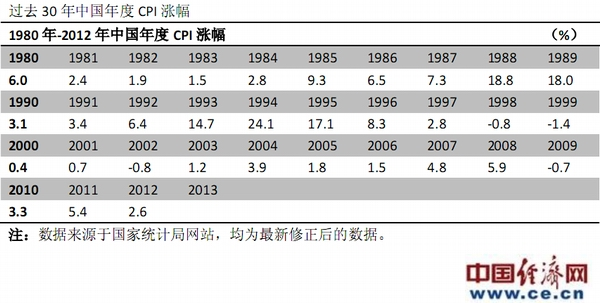
\includegraphics[width=\linewidth]{tongpeng30.jpg}
  \caption[1980--2012年CPI通膨率]{\label{fig:tongpeng30}注:图中CPI涨幅为本年相较
    上一年的涨幅。 }
  \capsource{\url{http://intl.ce.cn/specials/zxxx/201308/09/t20130809_24648757.shtml}}
\end{figure}

截止到1988年价格闯关前,通货膨胀所收取的高额通货膨胀暗税或铸币暗税;1985--1987一
些社会事件;粮食合同定购农民积极性持续下滑,以至于发展到1990年国家要实行强制性更
强的“国家定购”才能完成中央收购;党中央在邓小平、赵紫阳的主导下决定尽快双轨并轨
为市场一轨,实行激进“物价、价格闯关”的主因——“双轨制价格造成的腐败和经济秩序混
乱”——也被他们无视掉了;1988年人民恐慌挤兑抢购的事实何在,只是因为激进的价格闯关
来临,就没有之前“温和的”价格双轨制所造成的原因吗?张维迎、张曙光等对双轨制的辩
护中,他们认为计划轨的失败,本就属于双轨制改革的目的。计划轨的废除本就是目的,那
么主要依赖计划轨的民众怎么办呢?他们居然说这是无损于弱势一方福利的帕累托改进!

最后,理论方面,帕累托改进局限在哪里?真的会有一方利益无损而另一方利益可以尽情增
长的帕累托改进吗,它是真命题吗?笔者对西方经济学并不了解,以相当轻率和主观臆测的
态度找到几篇论文,供读者阅读,并希望读者积极回馈你们想法,尤其是对读者的批判和交
流。\footnote{既然态度看似如此草率,为何笔者还要提出以下内容呢?因为民为贵,社稷
  次之,君为轻,而能贯行此道的文章甚少,它们孤冷而不易。笔者甘冒鲁莽、幼稚、狂妄
  的错误尽可能去发掘这些文章。笔者多提几篇文章,若在此类文章中实则只有寥寥几篇此
  道好文笔者也觉欣慰。}价格双规制中帕累托改进的理论错误:张军《价格双轨制:是奇迹
还是神话》\footnote{http://economics.efnchina.com/show-1554-58760-1.html};帕累托
改进的各方局限性:姚洋《作为一种分配正义原则的帕累托改进》\cite{yaoyang};帕累托
改进理论的伪命题:朱富强《帕累托改进原则能否应用于社会改革?——实践的可行性和内在
的保守性》\cite{zhufuqiang},宋圭武《“帕累托最优”质疑》\cite{songguiwu}。

据国际货币基金组织《国际金融统计》和数据文件,1987年CPI通胀率较上年上
升7.234\%,1988年较上一年上升18.812\%,1989年较上一年上升18.246\%。

杨继绳\cite{yangshuanggui}和张曙光就李鹏向邓小平反映价格问题的时间有出入,杨继绳
说是七届全国人大一次会议期间,张曙光说是两会后,笔者认为并没有实质的差别,以下以
张曙光记述为准。
\begin{quotation}
  1988年3月25日到4月13日,一年一度的“两会”在北京召开,物价和‘官倒’问题成为会
  议议论的焦点。代表们强烈抨击双轨制给不法分子可乘之机,痛斥社会风气每况愈下。

  两会后,李鹏向邓小平汇报会议情况。邓小平问代表们意见最大的是什么事情,李鹏说是
  价格问题,双轨价格造成的腐败和经济秩序混乱。邓小平再次提出要闯过价格改革这一关。
  并认为“\textbf{晚过不如早过}”、“\textbf{长痛不如短痛}”。事后,李鹏向中央政
  治局传达了邓小平价格闯关的意见。\pagescite[][563]{fengyunshi1b}
\end{quotation}

1988年8月15日至17日,中共中央政治局在北戴河召开第十次全体会议,通过了《关于价格、
工资改革的初步方案》,价格闯关正式开始,部分烟酒市场价较原来提高10倍,全国挤兑抢
购现象相当严重。1989年2月,CPI通胀率同比(去1988年2月相比)增长28.4\%,为改革开放
以来同比最高比例。

1988年因价格闯关彻底失败,保守派势力处于上升趋势,自由派势力相当之前有所减弱。同
年9月26日至30日,中共十三届三中全会召开,“会议批准了中央政治局向这次全会提出
的\textbf{治理经济环境、整顿经济秩序、全面深化改革}的指导方针和政策、措施。……治
理经济环境,主要是压缩社会总需求,抑制通货膨胀。整顿经济秩序,就是要整顿目前经济
生活中特别是流通领域中出现的各种混乱现
象。
”\footnote{\url{http://cpc.people.com.cn/GB/64162/64165/70293/70319/4857100.html}}

\begin{quotation}
  由于连续两年的治理整顿,再加上1989年的政治风波,中国的经济运行发生了重大变化,
  从经济过热变成增长过慢,从通货膨胀变成通货紧缩。1988年和1989年GDP分别增
  长4.1\%和3.8\%,1990年和1991年零售物价上涨率从1988年的18.5\%和1989年的17.8\%下
  降到1990年的2.1\%和1991年的2.9\%。市场秩序也发生了逆转,从紧张变成疲软,从旺销
  变成滞销,持续了几十年的卖方市场第一次出现了买方市场,这就导致了计划内外价差的
  缩小,计划价格变成了市场价格。于是,双规价格自然而然地实现了并轨,到1991年底,
  80\%的商品价格都已经放开,基本上实现了市场化。这真是“踏遍铁鞋无觅处,得来全不
  费功夫”。\pagescite[][579]{fengyunshi1b}
\end{quotation}
笔者想,一些领导人和西方主流经济学家极力推动,举国之力想要完成的事情都没有完成,
却被历史和真正市场(并非以现代西方经济学所应用的市场)以一种荒谬、戏谑众生和神奇
的自我调节方式实现了最终的并轨……


\section{金融改革}
\label{sec:huilv78}

\subsection{现代化银行}

1979年10月4日,邓小平同志在省、自治区、直辖市党委第一书记座谈会上作出讲话,收录在
《关于经济工作的几点意见》。意见中指出:“必须把银行真正办成银行……过去我们的制
度是采取拨款的形式,而不是银行贷款的形式。这个制度必须改革。任何单位要取得物资,
要从银行贷款,都要付利息。”我国开始了恢复、重构金融体系的工作。

1979年到1984年,中国恢复和建立了中国农业银行、中国银行、中国建设银行等专业银行,
中央人民银行专门行使中央银行职能,成立中国工商银行,承担原来由人民银行办理的工商
信贷和储蓄业务。同期也成立了中国国际信托投资公司和地方信托投资公司、租赁公司、农
村和城市信用合作社等。

1985年后,中央政府按照市场化运作的原则成立了一批股份制商业银行,包括交通银行、中
信实业银行、华夏银行等。

1986年12月19日,邓小平同志在听取中央负责同志汇报时再次指出“要把银行真正办成银行。
我们过去的银行是货币发行公司,是金库,不是真正的银行。对金融问题,我们知识不足,
可以聘请外国专家做顾问嘛”。


\subsection{汇率双轨制}

杨帆将市场经济过渡时期的汇率制度变革分为两个阶段。\cite{huilvshi}

20世纪70年代后期,因人民币汇率被严重高估,\textbf{全国平均出口换汇成本
  较官方汇率过高,造成企业出口越多亏损越大。}笔者根据杨帆文中表格测
算,1975--1979年的出口平均换汇成本均高于同期官方汇率50\%以上,最高达至68\%。

1978年8月为促进出口,平衡外汇收支,我国开始实行\textbf{外汇留成制},所谓“外汇留
成,即是对外贸易单位和出口生产企业把收入的外汇卖给国家,国家按一定比例拨给他们相
应的外汇留成。”

\begin{quotation}
  “外汇留成有两种形式,一种是\textbf{现汇}(在企业和地方、国家间直接分配外汇数量),一
  种是\textbf{额度};且以后者为主。所谓外汇额度,是指按照官方汇率获取外汇的一种权
  利。其目的是\textbf{政府直接控制外汇},其办法是,外贸企业必须将\textbf{包括留成
    外汇在内的全部收汇,按官方价格售给政府指定的银行,}同时按照留成比例拿到一个凭
  证,即\textbf{外汇额度}。当该企业想使用外汇时,再持\textbf{外汇额度凭证}到银行
  按照政府规定的汇率用人民币购买外汇”。\pagescite[][769]{fengyunshi1b}
\end{quotation}


杨帆将1981年至1984年间划分为转轨时期第一阶段——“\textbf{人民币内部结算价和官方汇
  率并存的双重汇率时期}”。此一时期,\textbf{贸易内部结算价}基本不变,“贸易内部
结算价按照1978年全国平均换汇成本2.53人民币/美元加上\textbf{10\%的出口利润}计算出
来,为2.8人民币/美元……我国贸易收支明显好转,外汇储备明显增加。\textbf{1984年外
  汇储备年末累计余额170.42亿元特别提款权,为历史上和20世纪80年代最高水平”}。

\begin{quotation}
  有外汇额度的企业暂时不用,而没有外汇额度的企业却急需用汇,外汇额度交易
  (\textbf{合法和非法})及其交易场所就应运而生。\pagescite[][769]{fengyunshi1b}
\end{quotation}

1980年到1983年中国银行先后在北京、上海等12个城市开办了外汇调剂业务。张曙光指出,
调剂柜台\textbf{外汇交易价格}为贸易内部结算价2.8人民币/美元基础上上浮10\%,(蛋蛋
注:即3.08人民币/美元),但这仍然低于\textbf{市场影子价格}。

\begin{quotation}
  随着外汇留成的增加和官方控制的放松,\textbf{私下的场外交易}发展起来……一美元可
  以兑付4--5元人民币\footnote{原书此处为4--5美元,笔者认为明显是张曙光笔误,但这
    一时期完善资料数量少,又常常埋没在诸多平庸论述中,难以查证。如有错漏还望读者
    批评指正。}。这样,外汇额度的价值已经由\textbf{市场}来评价了。\textbf{一般的
    交易方式}是,(蛋蛋注:有外汇额度凭证的企业)先在银行按照官价提取外汇,出门后
  再按\textbf{黑市价格}补齐(蛋蛋注:按黑市价格卖给需求外汇的企业或个人
  )。\pagescite[][769]{fengyunshi1b}
\end{quotation}

杨帆提及“(第一阶段)影响了\textbf{非贸易部门}的积极性……\textbf{外贸亏损增大},
在对外经济中陷入被动,造成了\textbf{外汇管理的混乱},更加重了\textbf{国家的财政负
  担}。因此实行内部结算价注定成为一个\textbf{过渡时期的应急措施}。”

杨帆将1985--1993年间划分为转轨时期的第二阶段:
\begin{quotation}
  \textbf{官方汇率}和\textbf{外汇调剂市场汇率}并存时期。 从1985年1月1日起,我
  国\textbf{取消内部结算价},官方汇率应用于\textbf{贸易结算}和\textbf{非贸易外汇
    兑付}。

  为\textbf{鼓励出口},在\textbf{人民币汇率下调}的同时,1985年国家又一
  次\textbf{提高外汇留成比例},采取按出口商品收汇金额比例留成的办法。
\end{quotation}
这一阶段官价实行以美元为基准的有限弹性汇率制。综合来看汇率恰逢其时的步入
了\textbf{实质性和典型的价格“双轨制”时期}。

\begin{quotation}
1988年上海首创外汇调剂公开市场,实行公开竞价制度,其它城市也纷纷效仿。这样一来,
外汇现汇交易和额度交易就\textbf{合法化}了。\pagescite[][769-770]{fengyunshi1b}

1988年后,国家\textbf{放开了外汇调剂价格},调剂价格根据外汇供求\textbf{自由浮动}。
同年,在北京设立了\textbf{全国外汇调剂中心},形成了全国统一的外汇调剂市
场。\cite{wangqiangshehui}

1988年我国外贸体制进行了重大改革,外贸开始推行承包责任制,并对轻工、工艺、服装三
个行业实行独立核算、自负盈亏。1991年外贸由补贴机制转向自负盈亏机制,取消财政补贴。
外贸体制改革的深化,要求人民币汇率成为调节进出口贸易的主要手段。

1988年至1993年由于\textbf{经济过热、通货膨胀}、物价上涨、进口需求猛增(蛋蛋注:据
管涛,1993年,中国出现了历史上最后一次年度贸易逆差。),外汇\textbf{求大于供},市
场汇率\textbf{不断下跌},由5.70/美元贬值为1993年2月的8.20人民币/美元。为
了\textbf{限制汇率投机性上涨},一度实行限价,造成\textbf{外汇流向场外交
  易}。1993年5月\textbf{取消限价},市场汇率骤升至\textbf{11.20人民
  币/美元}。1993年7月以后,在国家加强宏观调控和中国人民银行对市场进行干预下,
到1993年底市场汇率回落到\textbf{8.72人民币/美元}。\cite{huilvshi}

从1994年1月1日起,国家决定实行\textbf{单一的有管理的浮动汇率制},实现了官方汇率与
调剂市场汇率的并轨。特别要强调的是,1994年汇率并轨时,人民币汇率制度是\textbf{以
  市场供求为基础的、 单一的、有管理的浮动汇率制度}。其中,这个“单一”\textbf{不
  是单一盯住美元的汇率制度},而是相对于1994年并轨以前的双重汇率制度来说的。双重汇
率制度时期,官方汇率和外汇调剂市场汇率的差价很大,并轨以后,所有的交易都使用
了\textbf{市场形成的汇率},因此,强调了“\textbf{单一}”。\cite{guantaohuigai}
\end{quotation}

市场经济体制过渡时期的汇率双轨思路是一贯的,国家抛弃财政包袱,减少对各方面投入和
支持,获取收益,解决原来企业出口亏损问题,通过汇率双轨、特别是持续增加市场一轨的
权重刺激出口,做大市场。改革过程中出现的问题也是简明的,同农业、企业方面的双轨制
一样,计划轨外市场一轨的融入所实行的双轨制,增大了黑市的操作空间,需要注意的是,
这里的黑市主体不是民间个人,而是权力拥有或相关的个人或企业。双轨制似乎是势在必行
的,权力寻租似乎也是无法避免的。笔者认为,这可能是历史的趋势吧,不以个人或组织甚
至国家主观意愿为转移的趋势。但笔者也认为,不管负面影响是不是大势所趋,在任何政策
的制定和执行过程中,不能因为负面影响不可避免,就忽视负面程度上的大
小,这已经成为当代学者和政治家的通病。\improve[inline]{是不是将结论放到本章结尾再行论述呢?只展示资料?}

\section{财政体制改革}

\subsection{财政体制改革的深层逻辑}

2008年3月18日,时任国务院总理温家宝在十一届全国人大一次会议的记者见面会上说:“其
实一个国家的财政史是惊心动魄的。如果你读它,会从中看到不仅是经济的发展,而且是社
会的结构和公平正义。”

\begin{quotation}
  回顾40年改革长路,是什么在推动中国财政改革?其深层逻辑又是什么?我们发现,从过
  去到现在,这一问题根本上可以归结为一点,那就是公共风险的变化。\textbf{财政改革
    往往不是在先见之明的制度设计基础上进行的,而是在公共风险暴露与加剧时,不得不
    做出的选择。}

   防范和化解公共风险是财政改革的原动力。从历史上看,制度变迁无一不是公共风险与
  危机推动的结果,而制度变迁的突破口常常是在财政。改革开放以来,我国财政改革实质
  上都是遵循公共风险变化的逻辑而推进的,其变化的脉络是从“\textbf{家贫国穷}”的风
  险到“\textbf{机会不均}”的风险,再到\textbf{全球公共风险},这也是我国主要公共
  风险的昨天、今天和明天。
\end{quotation}


\subsection{税制改革}

1980年9月10日,第五届全国人民代表大会第三次会议通过了《中华人民共和国中外合资经
营企业所得税法》和《中华人民共和国个人所得税法》。1981年12月13日,第五届全国人民
代表大会第四次会议通过了《中华人民共和国外国企业所得税法》。中国涉外税制初步建立。

1980年2月,国务院颁发了《关于实行"划分收支,分级包干"的财政管理体制的规定》,全面
推行包干式财政管理体制,扩大地方财政权限,俗称“分灶吃饭”,改变了过去“统收统
支”的财政体制。这一政策实行至1984年。

1983年进行了国有企业上交利润转上交税收的第一步改革,小型国有企业自负盈亏。1984年
进行了第二步利改税改革,进一步分解增设多种税种,由税利并存逐步过渡到完全的以税代利。

1985年3月21日,国务院发布《关于实行“划分税种、核定收支、分级包干”的财政管理体制
的规定》,进一步改革包干式财政管理体制,“一定五年不变”。

税制改革从此成为中央与地方政府的博弈场。依马骏所说,原“分灶吃饭”税制
中,“20\%共享收入归地方的一刀切计算办法使富省多有结余,穷省多有赤字”,因此促成
了这次改革。新税制改革的弊端是:
\begin{quotation}
  自1978年底以来,政府财政收入占国民生产总值的比例及中央财政收入占全部财政收入的
  比重快速地下降。

  (地方政府)利用各种减免税来调节其实际税收努力……地方政府对有效税率及税基的控
  制还表现在其对财政收入渠道的控制……地方政府预算内收入比重的下降和预算外收入上
  升,中央政府控制全国财政收入与支出的能力相应下降。

  由于地方政府在事实上控制了有效税率和税基,中央政府越来越多地依赖于一些不规范的
  政策工具来控制地方向中央上缴的财政收入。\cite{majuncaigai}
  \improve[inline]{分税制也要借鉴这篇文章}
\end{quotation}

财政部官网转载刘邦驰、马韵《三十年税制改革的回顾与发展趋向》\footnote{\url{http://www.mof.gov.cn/zhuantihuigu/czgg0000_1/czggcz/200811/t20081106_88385.html}}
,将1978年--1993年这一时期的税制改革称为“有计划商品经济时期的税制改革”,涉外
税制、利改税(“新中国成立后实行了30多年的国营企业向国家上缴利润的制度改为缴纳
企业所得税和调节税”)、个人所得税等税务改革。
\begin{quotation}
  这一时期全面改革了工商税制,建立了涉外税制,彻底摒弃了“非税论”和“税收无
  用论”的观点,恢复和开征了一些新税种,从而使我国税制逐步转化为多税种、多环
  节、多层次的复合税制,税收调节经济的杠杆作用日益加强。\footnote{\url{http://finance.ce.cn/sub/2013zt/zgszgg/hgyzw/201304/18/t20130418_199980.shtml}}
\end{quotation}

\improve[inline]{中央与地方张力,税务历史、}

\subsection{拨改贷}

1985年,所有国家基本建设投资由财政无偿拨款改为向中国人民建设银行贷款,并要还付本
息,即“拨改贷”。信托投资公司兴起。
\begin{quotation}
  1984年国家出台拨款改贷款政策后,意味着1984年以后新成立的国企,一出生就是
  100\%的负债率。\cite{bogaidaizhaizhuangu}

  国有企业高负债率的直接原因是国家在1983年实行了拨改贷,对国有企业的投资由财政拨
  款改为向银行的贷款。国有企业高负债率的间接原因则是国有企业的预算软约
  束\footnote{软预算约束就是指当一个经济组织遇到财务上的困境时,借助外部组织的求
    助得以继续生存这样一种经济现象。}。\cite{linyifuzhai}

  银行系统贷给国有企业的贷款很多都成了呆坏账,国有企业拖欠还贷的情况非常严重。但
  是,出于对国有企业进行政策性支持的需要,银行在政府的影响下,会继续向那些企业发
  放贷款。这样日积月累,便形成了银行系统今天巨额的不良资产。(林毅夫与李志赟就此
  总结有三个原因,一是计划经济转入市场经济过程中,原资本密集型国有企业尤其受到外
  资、合资企业冲击,由此造成的战略性政策负担;二是国有企业承担了大量劳动力的养老、
  医疗、教育等社会保障责任,由此造成的社会性政策负担;三是无法划清亏损企业经营者
  的责任,经营者往往将责任归咎于前两者,并以此为理由拖欠银行贷款,政府在各方面压
  力下干预银行,要求银行继续贷款给亏损企业,由此造成预算软约束问题
  。)\cite{guoyoujinrong}
\end{quotation}

\improve[inline]{由“拨改
  贷”到“债转
  股”\url{http://www.hprc.org.cn/gsyj/jjs/jjyxs/201702/t20170220_388850.html}}


\section{权力寻租、官倒和腐败}

\subsection{历史政策}
陈云 \url{http://cpc.people.com.cn/GB/69112/83035/83317/83597/5738412.html}《经济形势与经验教训 (一九八〇年十二月十六日)》

1981年1月7日,国务院《关于加强市场管理、打击投机倒把、走私贩私活动的指示》
1982年4月10日政治局会议讨论《中共中央、国务院关于打击经济领域中严重犯罪活动的
决定》。4月13日,中共中央、国务院发布了《关于打击经济领域中严重犯罪活动的决定》。
1983年9月15日,人民日报发表评论员文章《必须依法从重从快惩处经济罪犯》。1983年
月12日,中共第十二次全国代表大会发出《中共中央关于整党的决定》。1984年12月3日,
中共中央、国务院发出《关于严禁党政机关和党政干部经商、办企业的决定》。1985年5月
23日,中共中央、国务院发出《关于禁止领导干部的子女、配偶经商的决定》。1986年2月
日,中共中央、国务院发布《关于进一步制止党政机关和党政干部经商、办企业的决定》。
1989年2月5日,中共中央办公厅、国务院办公厅发出《关于清理党和国家机关干部在公司
(企业)兼职有关问题的通知》。

关于价格双轨制时期的腐败请见\cref{sec:qishuanggui}。

% 1983年8月,全国政法工作会议公布《中共中央关于严厉打击刑事犯罪活动的决定》,全
% 国从重从速严打刑事犯罪。

改革开放之后,权力寻租和腐败问题便浮出水面,贯穿这一时期始终,并未得到有效治理。
有专家学者认为权力问题成为这一时期价格双轨制、利改税、拨改贷等政策负面作用巨大的主
要原因。个别专家甚至认为正是改革开放实际实行的体制产生了权力失控,从而导致权贵资
本主义的形成和腐败,并且权贵资本资本主义将导致中国政体的溃败。比如孙立
平\cite{sunlipingkuibai}、钱理群\cite{maohehoumao2}等。


% \begin{verbatim}
% https://www.modernchinastudies.org/us/issues/past-issues/45-mcs-1995-issue-1/253-2011-12-29-11-30-06.html
% 中央与地方财政关系的改革

% 南方周末:重议分税制——分钱还是分权? https://www.guancha.cn/economy/2013_08_15_165993.shtml

% 分税制的是与非 http://liushangxi.blog.caixin.com/archives/60712

% http://www.sss.net.cn/112/65928.aspx
% 刘尚希:财政改革四十年的深层逻辑

% 回顾40年改革长路,是什么在推动中国财政改革?其深层逻辑又是什么?我们发现,从过去到现在,这一问题根本上可以归结为一点,那就是公共风险的变化。财政改革往往不是在先见之明的制度设计基础上进行的,而是在公共风险暴露与加剧时,不得不做出的选择。

%  防范和化解公共风险是财政改革的原动力。从历史上看,制度变迁无一不是公共风险与危机推动的结果,而制度变迁的突破口常常是在财政。改革开放以来,我国财政改革实质上都是遵循公共风险变化的逻辑而推进的,其变化的脉络是从“家贫国穷”的风险到“机会不均”的风险,再到全球公共风险,这也是我国主要公共风险的昨天、今天和明天。

% http://www.cssn.cn/zx/bwyc/201806/t20180626_4421303.shtml
% 中央、地方与企业:财政体制改革40年

% http://theory.people.com.cn/GB/49154/49155/8094994.html

% http://www.pkulaw.cn/fax/czf/contents/class02_3_1r.htm

% http://www.hprc.org.cn/gsyj/jjs/jjyxs/201702/P020170220376223183282.pdf
% 贷改投

% http://www.ccswf.org.tw/files/7100/18/%E5%AD%90%E9%A1%8C3-2%E8%94%A1%E7%A6%BE.pdf

% https://www.guancha.cn/HuAnGang/2014_04_27_224728.shtml
% 分税制改革二十年后

% 建国以来最高通货膨胀是什么时候?
% 19 9 4 年物价 上 涨超 过 2 0 \% , 成为 改革 以来通 货膨 胀 最严 重 的年份
% . 市
% http://img.bimba.pku.edu.cn/res/download/ceq/1_4/010405.pdf

% http://www.chinagrain.cn/axfwnh/2018/09/19/1511534741.shtml
% 我国粮食收储体制改革的历程、体制性问题分析及改革的方向与对策建议

% http://www.china.com.cn/chinese/EC-c/50868.htm  重要粮食流通体制改革:双轨过渡与双轨终结
% \end{verbatim}

% ( 4) 共产主义社会高级阶段。 中国共产党第十三次全国代表大会的报告中指出, 社会主义初级阶% 段 “ 不是泛指任何国家进入社会主义社会都会经历的起始阶段, 而是特指我国在生产力落后、 商品% 经济不发达条件下建设社会主义必然要经历的特定阶段 。” [6 ] % 发达资本主义国家在无产阶级夺取 出自《正确认识和对待“共产主义渺茫论”》
% \improve[inline]{\url{http://theory.people.com.cn/GB/148980/16813293.html},邓小
%   平南巡的三个坚定不移。}


%%% Local Variables:
%%% mode: latex
%%% TeX-master: "../main"
%%% End:
